% hack to deal with beamer/pgf bug
\RequirePackage{atbegshi}

% "draft" makes compilation faster; remove for final version
% shadow = put drop shadows behind blocks by default
% xcolor: svgnames imports lots of color names
% table allows for multi-color table rows
% pdftex is the compiler
\documentclass[shadow,xcolor=pdftex,svgnames,table,t]{beamer}

\usepackage{amsmath,amssymb,amsfonts}

% need to load tikz defs before beamer defs, for some reason
% additional libraries for tikz and pgf
\usepackage{tikz}
\usetikzlibrary{matrix}
\usetikzlibrary{calc}
\usetikzlibrary{shadows}
\usetikzlibrary{scopes}
\usetikzlibrary{chains}
\usetikzlibrary{positioning}
\usetikzlibrary{fit}
\usetikzlibrary{backgrounds}
\usetikzlibrary{decorations.pathmorphing}
\usetikzlibrary{decorations.pathreplacing}
\usetikzlibrary{shapes.geometric}
\usetikzlibrary{shapes.symbols}
\usetikzlibrary{shapes.misc}
\usetikzlibrary{trees}

% color aliases
%\colorlet{Lattice}{Green}
%\colorlet{Set}{Red!10}

% global styles
\tikzset{
  % make drop shadows a bit softer
  every shadow/.style={opacity=.4,shadow xshift=.3ex,shadow yshift=-.3ex},
  % use \& to separate cells in matrices, avoiding fragility in beamer frames
  every matrix/.style={ampersand replacement=\&},
  % edges and joins with arrows and thicker
  every edge/.append style={->,thick},
  every join/.style={->,thick},
  % distance between nodes
  % node distance=1ex and 2ex,
}

% styles for drawing in Rn, especially lattices
\tikzset{
  % lattice transform must include "cm" dimension to work properly,
  % otherwise the x and y transforms become dependent
  Ztrans/.style={x={(1.5cm,1cm)},y={(.5cm,1.5cm)}},
  Zdual/.style={x={(1.5cm,-.5cm)},y={(.5cm,1cm)}},
  latttrans/.style={x={(1.8cm,.5cm)},y={(0.4cm,1.3cm)}},
  dualtrans/.style={x={(1.3cm,-.4cm)},y={(-.5cm,1.8cm)}},
  lattB/.style={x={(1.8cm,.5cm)},y={(0.4cm,1.4cm)}},
  dualB/.style={x={(1.4cm,-.4cm)},y={(-.5cm,1.8cm)}},
  shortB/.style={x={(.5cm,.2cm)},y={(-.1cm,1.7cm)}},
  latt2B/.style={x={(1cm,.1cm)},y={(.1cm,1.2cm)}},
  ulattB/.style={x={(2.0cm,.5cm)},y={(2.1cm,-.2cm)}},
  openball/.style={fill=structure.fg!20},
  ball/.style={openball,thin,draw=structure.fg},
  latt/.style={Lattice,fill},
  dist/.style={Brown,densely dashed,font=\footnotesize},
  offlabel/.style={Brown,inner sep=2pt,font=\tiny},
  axes/.style={->,Gray,style=very thin},
  fundamental/.style={Gray,fill opacity=.2},
  target/.style={fill,Brown},
  project/.style={thin,dashed},
  help lines/.style={Gray,very thin,step=.5cm},
  % expanding waves representing noise
  noise/.style={
    Lattice,
    opacity=.5,
    decorate,decoration={
      expanding waves,
      segment length=5pt,angle=10,
      post=moveto,post length=3pt
    },
  },
}

% lattice that can be dropped into any path.
% it would be sensible to set a default argument here, but
% commands with optional args don't parse correctly inside a
% tikz path
\newcommand*{\latt}[1]{%
  \foreach \a in {-4, ..., 4} {
    \foreach \b in {-4, ..., 4} {
      (\a,\b) circle (#1)
    }
  }
}

% style for functions mapping one point to another
\tikzset{map/.style={->,semithick}}

% style for an offset rounded box
\tikzset{showoff/.style={draw,fill=White,rounded corners,drop
    shadow,inner sep=6pt}}

% style for all algorithms
\tikzset{algorithm/.style={
    draw=#1!50!Black!60,solid,
    top color=White,bottom color=#1!50!Black!15,
    very thick,rounded corners,drop shadow,
    minimum size=.9cm,inner sep=6pt,outer sep=4pt
  }
}

% style for honest, malicious, trusted parties
\tikzset{honest/.style={algorithm=Green}}
\tikzset{oracle/.style={algorithm=Green}}
\tikzset{malicious/.style={algorithm=Red}}
\tikzset{trusted/.style={algorithm=Purple,inner sep=10pt}}

% style for notions
\tikzset{notion/.style={
    draw=#1!50!Black!60,solid,
    top color=White,bottom color=#1!50!Black!15,
    very thick,rounded corners,drop shadow,
    minimum height=6.5ex,inner sep=6pt,
  }
}

\tikzset{app/.style={notion=Blue}}
\tikzset{prim/.style={notion=Green}}
\tikzset{math/.style={notion=Red}}

% % style for a common reference string
\tikzset{crs/.style={draw,fill=White,cloud,cloud puffs=13,cloud ignores aspect,drop shadow}}

%% BOILERPLATE PRESENTATION STUFF

% an underlining package
\usepackage{ulem}
% use normal italics for emphasis
\normalem

% my custom theme
\usetheme{CJP}

% dingbats
\usepackage{pifont}

\renewcommand{\Check}{\ding{52}}
\newcommand{\Cross}{\ding{55}}
\newcommand{\Hand}{\ding{43}}
\newcommand{\GreenCheck}{{\color{Green}\Check}}
\newcommand{\RedCross}{{\color{Red}\Cross}}
\newcommand{\Orange}[1]{{\color{Orange} #1}}

% alias for citations
\newcommand{\citationsize}{\footnotesize}

\subject{Theoretical Computer Science}

% suppress ugly QEDs in proofs
\def\qedsymbol{}


% common stuff
% basic notation

\newcommand{\lamperp}{\Lambda^{\perp}}
\newcommand{\lam}{\Lambda}

% lattice
\newcommand{\lat}{\mathcal{L}}
% fundamental region
\newcommand{\piped}{\mathcal{P}}
% smoothing parameter
\newcommand{\smooth}{\eta}
% smoothing w/ epsilon
\newcommand{\smootheps}{\smooth_{\epsilon}}
% ball
\newcommand{\ball}{\mathcal{B}}
% cube
\newcommand{\cube}{\mathcal{C}}
% covering radius symbol
\newcommand{\cover}{\ensuremath{\mu}}
% Gram-Schmidt
\newcommand{\gs}[1]{\ensuremath{\widetilde{#1}}}
% GS minimum
\newcommand{\gsmin}{\ensuremath{\tilde{bl}}}
% volume operation
\DeclareMathOperator{\vol}{vol}
% Hermite normal form
\DeclareMathOperator{\hnf}{HNF}
% rank
\DeclareMathOperator{\rank}{rank}
% distance operator
\DeclareMathOperator{\dist}{dist}
% span operator
\DeclareMathOperator{\spn}{span}
% error function
\DeclareMathOperator{\erf}{erf}

% quantities that show up regularly
\newcommand{\wsln}{\ensuremath{\omega(\sqrt{\log n})}}
\newcommand{\wslm}{\ensuremath{\omega(\sqrt{\log m})}}

% support algorithms
\newcommand{\sampleZ}{\algo{Sample}\Z}
\newcommand{\sampleD}{\algo{SampleD}}
\newcommand{\tobasis}{\algo{ToBasis}}
\newcommand{\invert}{\algo{Invert}}
\newcommand{\genbasis}{\algo{GenBasis}}
\newcommand{\extbasis}{\algo{ExtBasis}}
\newcommand{\extlattice}{\algo{ExtLattice}}
\newcommand{\randbasis}{\algo{RandBasis}}
\newcommand{\gentrap}{\algo{GenTrap}}
\newcommand{\deltrap}{\algo{DelTrap}}
\newcommand{\noisy}{\algo{Noisy}}

% problems related to lattices
\newcommand{\svp}{\problem{SVP}}
\newcommand{\gapsvp}{\problem{GapSVP}}
\newcommand{\cogapsvp}{\problem{coGapSVP}}
\newcommand{\usvp}{\problem{uSVP}}
\newcommand{\sivp}{\problem{SIVP}}
\newcommand{\gapsivp}{\problem{GapSIVP}}
\newcommand{\cvp}{\problem{CVP}}
\newcommand{\gapcvp}{\problem{GapCVP}}
\newcommand{\cvpp}{\problem{CVPP}}
\newcommand{\gapcvpp}{\problem{GapCVPP}}
\newcommand{\bdd}{\problem{BDD}}
\newcommand{\gdd}{\problem{GDD}}
\newcommand{\add}{\problem{ADD}}
\newcommand{\incgdd}{\problem{IncGDD}}
\newcommand{\incivd}{\problem{IncIVD}}
\newcommand{\crp}{\problem{CRP}}
\newcommand{\gapcrp}{\problem{GapCRP}}
% problems on ideal lattices
\newcommand{\igvp}{\problem{IGVP}}
\newcommand{\incigvp}{\problem{IncIGVP}}
% avg-case stuff
\newcommand{\sis}{\problem{SIS}}
\newcommand{\isis}{\problem{ISIS}}
\newcommand{\ilwe}{\problem{ILWE}}
\newcommand{\lwe}{\problem{LWE}}
\newcommand{\rlwe}{\problem{RLWE}}
\newcommand{\lwr}{\problem{LWR}}
\newcommand{\rlwr}{\problem{RLWR}}
\newcommand{\dlwe}{\problem{DLWE}}
\newcommand{\lpn}{\problem{LPN}}
\newcommand{\Psibar}{\ensuremath{\bar{\Psi}}}

% macros for matrices and vectors
\newcommand{\matA}{\ensuremath{\mathbf{A}}}
\newcommand{\matB}{\ensuremath{\mathbf{B}}}
\newcommand{\matC}{\ensuremath{\mathbf{C}}}
\newcommand{\matD}{\ensuremath{\mathbf{D}}}
\newcommand{\matE}{\ensuremath{\mathbf{E}}}
\newcommand{\matF}{\ensuremath{\mathbf{F}}}
\newcommand{\matG}{\ensuremath{\mathbf{G}}}
\newcommand{\matH}{\ensuremath{\mathbf{H}}}
\newcommand{\matI}{\ensuremath{\mathbf{I}}}
\newcommand{\matJ}{\ensuremath{\mathbf{J}}}
\newcommand{\matK}{\ensuremath{\mathbf{K}}}
\newcommand{\matL}{\ensuremath{\mathbf{L}}}
\newcommand{\matM}{\ensuremath{\mathbf{M}}}
\newcommand{\matN}{\ensuremath{\mathbf{N}}}
\newcommand{\matO}{\ensuremath{\mathbf{O}}}
\newcommand{\matP}{\ensuremath{\mathbf{P}}}
\newcommand{\matQ}{\ensuremath{\mathbf{Q}}}
\newcommand{\matR}{\ensuremath{\mathbf{R}}}
\newcommand{\matS}{\ensuremath{\mathbf{S}}}
\newcommand{\matT}{\ensuremath{\mathbf{T}}}
\newcommand{\matU}{\ensuremath{\mathbf{U}}}
\newcommand{\matV}{\ensuremath{\mathbf{V}}}
\newcommand{\matW}{\ensuremath{\mathbf{W}}}
\newcommand{\matX}{\ensuremath{\mathbf{X}}}
\newcommand{\matY}{\ensuremath{\mathbf{Y}}}
\newcommand{\matZ}{\ensuremath{\mathbf{Z}}}
\newcommand{\matzero}{\ensuremath{\mathbf{0}}}

\newcommand{\veca}{\ensuremath{\mathbf{a}}}
\newcommand{\vecalpha}{\ensuremath{\mathbf{\alpha}}}
\newcommand{\vecb}{\ensuremath{\mathbf{b}}}
\newcommand{\vecc}{\ensuremath{\mathbf{c}}}
\newcommand{\vecd}{\ensuremath{\mathbf{d}}}
\newcommand{\vece}{\ensuremath{\mathbf{e}}}
\newcommand{\vecf}{\ensuremath{\mathbf{f}}}
\newcommand{\vecg}{\ensuremath{\mathbf{g}}}
\newcommand{\vech}{\ensuremath{\mathbf{h}}}
\newcommand{\veck}{\ensuremath{\mathbf{k}}}
\newcommand{\vecm}{\ensuremath{\mathbf{m}}}
\newcommand{\vecp}{\ensuremath{\mathbf{p}}}
\newcommand{\vecq}{\ensuremath{\mathbf{q}}}
\newcommand{\vecr}{\ensuremath{\mathbf{r}}}
\newcommand{\vecs}{\ensuremath{\mathbf{s}}}
\newcommand{\vect}{\ensuremath{\mathbf{t}}}
\newcommand{\vecu}{\ensuremath{\mathbf{u}}}
\newcommand{\vecv}{\ensuremath{\mathbf{v}}}
\newcommand{\vecw}{\ensuremath{\mathbf{w}}}
\newcommand{\vecx}{\ensuremath{\mathbf{x}}}
\newcommand{\vecy}{\ensuremath{\mathbf{y}}}
\newcommand{\vecz}{\ensuremath{\mathbf{z}}}
\newcommand{\veczero}{\ensuremath{\mathbf{0}}}

\DeclareMathOperator{\diag}{diag}
\renewcommand{\O}{\mathcal{O}}

% "left-right" pairs of symbols

% inner product
\newcommand{\inner}[1]{\langle{#1}\rangle}
\newcommand{\innerfit}[1]{\left\langle{#1}\right\rangle}
% absolute value
\newcommand{\abs}[1]{\lvert{#1}\rvert}
\newcommand{\absfit}[1]{\left\lvert{#1}\right\rvert}
% a set
\newcommand{\set}[1]{\{{#1}\}}
\newcommand{\setfit}[1]{\left\{{#1}\right\}}
% parens
\newcommand{\parens}[1]{({#1})}
\newcommand{\parensfit}[1]{\left({#1}\right)}
% tuple, alias for parens
\newcommand{\tuple}[1]{\parens{#1}}
\newcommand{\tuplefit}[1]{\parensfit{#1}}
% square brackets
\newcommand{\bracks}[1]{[{#1}]}
\newcommand{\bracksfit}[1]{\left[{#1}\right]}
% rounding off
\newcommand{\round}[1]{\lfloor{#1}\rceil}
\newcommand{\roundfit}[1]{\left\lfloor{#1}\right\rceil}
% floor function
\newcommand{\floor}[1]{\lfloor{#1}\rfloor}
\newcommand{\floorfit}[1]{\left\lfloor{#1}\right\rfloor}
% ceiling function
\newcommand{\ceil}[1]{\lceil{#1}\rceil}
\newcommand{\ceilfit}[1]{\left\lceil{#1}\right\rceil}
% length of some vector, element
\newcommand{\length}[1]{\lVert{#1}\rVert}
\newcommand{\lengthfit}[1]{\left\lVert{#1}\right\rVert}


% blackboard symbols

\newcommand{\C}{\ensuremath{\mathbb{C}}}
\newcommand{\D}{\ensuremath{\mathbb{D}}}
\newcommand{\F}{\ensuremath{\mathbb{F}}}
\newcommand{\G}{\ensuremath{\mathbb{G}}}
\newcommand{\J}{\ensuremath{\mathbb{J}}}
\newcommand{\N}{\ensuremath{\mathbb{N}}}
\newcommand{\Q}{\ensuremath{\mathbb{Q}}}
\newcommand{\R}{\ensuremath{\mathbb{R}}}
\newcommand{\T}{\ensuremath{\mathbb{T}}}
\newcommand{\Z}{\ensuremath{\mathbb{Z}}}

\newcommand{\Zt}{\ensuremath{\Z_t}}
\newcommand{\Zp}{\ensuremath{\Z_p}}
\newcommand{\Zq}{\ensuremath{\Z_q}}
\newcommand{\ZN}{\ensuremath{\Z_N}}
\newcommand{\Zps}{\ensuremath{\Z_p^*}}
\newcommand{\ZNs}{\ensuremath{\Z_N^*}}
\newcommand{\JN}{\ensuremath{\J_N}}
\newcommand{\QRN}{\ensuremath{\mathbb{QR}_N}}

% trace
\DeclareMathOperator{\trace}{Tr}
\DeclareMathOperator{\lcm}{lcm}
\DeclareMathOperator{\msb}{msb}
\renewcommand{\O}{\mathcal{O}}
\newcommand{\frakp}{\mathfrak{p}}

% fix weird spacing of \pmod, and introduce \pmod* command; see
% http://tex.stackexchange.com/questions/39221/removing-extra-space-with-pmod-command
\makeatletter
\renewcommand{\pod}[1]{\mathchoice
  {\allowbreak \if@display \mkern 18mu\else \mkern 8mu\fi (#1)}
  {\allowbreak \if@display \mkern 18mu\else \mkern 8mu\fi (#1)}
  {\mkern4mu(#1)}
  {\mkern4mu(#1)}
}
\makeatletter
\let\@@pmod\pmod
\DeclareRobustCommand{\pmod}{\@ifstar\@pmods\@@pmod}
\def\@pmods#1{\mkern4mu({\operator@font mod}\mkern 6mu#1)}
\makeatother
%%%% 

\title
{ Practical Bootstrapping in\\Quasilinear Time
}

\author
{ {\Large Jacob Alperin-Sheriff}
  \and
  {\Large Chris Peikert}
}

\institute{School of Computer Science\\Georgia Tech}

\date
{
  UC San Diego\\
  29 April 2013
}

% restricts presentation to specified frames, for faster compilation;
% comment out the line to get the entire presentation

%\includeonlyframes{fhe,bootstrapping,results,unpacked-main}

\begin{document}

\begin{frame}[label=title]
  \titlepage
\end{frame}

\begin{frame}[label=fhe]{Fully Homomorphic Encryption {\footnotesize
      [RAD'78,Gen'09]}}
  \begin{itemize}
  \item<+-> FHE lets you do this:
    \begin{center}
      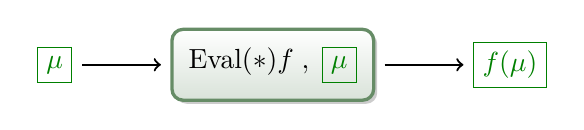
\begin{tikzpicture}
        \node (c) {$\color{Green}\fbox{$\mu$}$};
        \node[right=of c,algorithm=Green] (eval)
        {$\text{Eval}\parens*{f\;,\; {\color{Green} \fbox{$\mu$}}}$};
        \node[right=of eval] (out) {$\color{Green} \fbox{$f(\mu)$}$};

        \path
        (c) edge (eval)
        (eval) edge (out)
        ;
      \end{tikzpicture}
    \end{center}
    where $\abs{f(\mu)}$ and decryption time don't depend on
    $\abs{f}$.

    \medskip
    A cryptographic ``holy grail'' with tons of applications.
  \end{itemize}

  \onslide<+->
  \bigskip
  \begin{itemize}
  \item Naturally occurring schemes are ``somewhat
    homomorphic''~(SHE): they can only evaluate functions of an
    \alert<.>{\textit{a priori} bounded} depth.
  \end{itemize}

  \begin{center}
    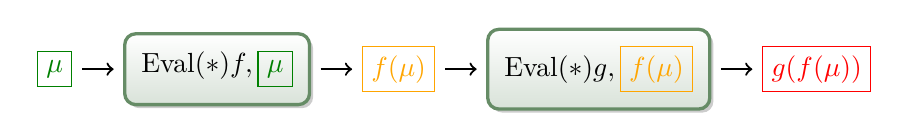
\begin{tikzpicture}[node distance=.4cm]
      \node (c) {$\color{Green}\fbox{$\mu$}$};
      
      \node[right=of c,algorithm=Green] (eval)
      {$\text{Eval}\parens*{f, {\color{Green} \fbox{$\mu$}}}$};
      
      \node[right=of eval] (cprime) {$\color{Orange} \fbox{$f(\mu)$}$};

      \node[right=of cprime,algorithm=Green] (eval2)
      {$\text{Eval}\parens*{g, {\color{Orange} \fbox{$f(\mu)$}}}$};

      \node[right=of eval2] (cdp) {$\color{Red} \fbox{$g(f(\mu))$}$};

      \path
      (c) edge (eval)
      (eval) edge (cprime)
      (cprime) edge (eval2)
      (eval2) edge (cdp)
      ;
    \end{tikzpicture}
  \end{center}
\end{frame}

\begin{frame}[label=bootstrapping]{Bootstrapping: SHE $\to$ FHE {\footnotesize [Gen'09]}}
  \begin{itemize}
  \item<+-> \alert<.>{Homomorphically evaluates the SHE decryption
      function} to ``refresh'' a ciphertext ${\color{Red}
      \fbox{$\mu$}}$, allowing further homomorphic operations.

    \begin{center}
      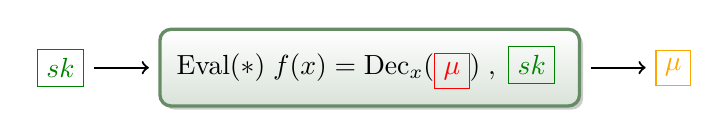
\begin{tikzpicture}[every node/.style={node distance=.7cm}]
        \node (sk)
        {${\color{Green} \fbox{$sk$}}$};

        \node[right=of sk,algorithm=Green] (eval)
        {$\text{Eval}\parens*{\; f(x) =
            \text{Dec}_{x}({\color{Red}\fbox{$\mu$}})\; ,\;
            {\color{Green} \fbox{$sk$}} \;}$};

        \node[right=of eval] (out)
        {${\color{Orange} \fbox{$\mu$}}$};

        \path
        (sk) edge (eval)
        (eval) edge (out)
        ;

      \end{tikzpicture}
    \end{center}

    \onslide<+->
    \begin{itemize}
    \item The only known way of obtaining \alert<.>{unbounded} FHE.

      \medskip
    \item \alert<.>{Goal}: Efficiency!  Minimize depth $d$ and
      size $s$ of decryption ``circuit.''

      \medskip
    \item Best SHEs {\footnotesize [BGV'12]} can evaluate in time
      $\tilde{O}(d \cdot s \cdot \lambda)$.
    \end{itemize}

    \smallskip

  \item<+-> Intensive study, many techniques {\footnotesize
      [G'09,GH'11a,GH'11b,GHS'12b]}, but

    \alert<.>{still very inefficient} -- the main bottleneck in FHE,
    by far.

    \medskip 
  
  \item<+-> The asymptotically most efficient methods on ``packed''
    ciphertexts {\footnotesize [GHS'12a,GHS'12b]} are very complex,
    and appear practically worse than asymptotically slower methods.

    % (No public implementation of sub-quadratic methods.)
  \end{itemize}
\end{frame}

\begin{frame}[label=great]{Milestones in Bootstrapping}
  \begin{description}
  \item<+->[[Gen'09{]}:] $\tilde{O}(\lambda^{4})$ runtime

    \medskip
  \item<+->[[BGV'12{]}:] $\tilde{O}(\lambda^{2})$ runtime, or
    $\tilde{O}(\lambda)$ amortized over $\lambda$ ciphertexts

    \onslide<+->
    \medskip
    Mainly via improved SHE homomorphic capacity.

    \medskip Amortized method requires ``exotic'' plaintext rings,
    emulating $\Z_{2}$ arithmetic in $\Z_{p}$.

    \medskip 
  \item<+->[[GHS'12b{]}:] $\tilde{O}(\lambda)$ runtime, for ``packed''
    plaintexts.  \alert<.>{Declare victory?}
  \end{description}
  %
  \onslide<+->
  \begin{center}
    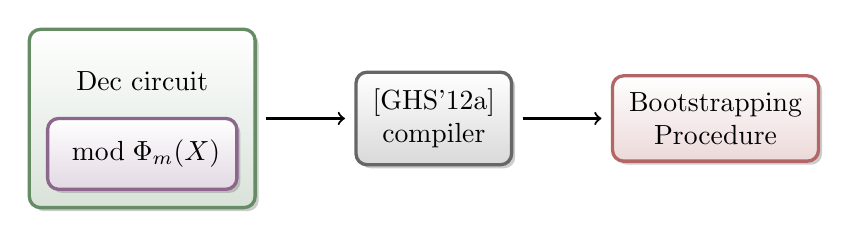
\begin{tikzpicture}
      \matrix[algorithm=Green] (Dec) {
        \node {Dec circuit}; \\
        \node[algorithm=Purple] (modPhi) {${} \bmod \Phi_{m}(X)$}; \\
      };

      \node[algorithm=Black,right=of Dec,align=center] (compiler)
      {[GHS'12a]\\compiler};

      \node[algorithm=Red,right=of compiler,align=center] (boot)
      {Bootstrapping\\Procedure};

      \path
      (Dec) edge (compiler)
      (compiler) edge (boot)
      ;
    \end{tikzpicture}
  \end{center}
  %
  \begin{itemize}
  \item<+->[\RedCross] Log-depth mod-$\Phi_{m}(X)$ circuit is
    \alert<.>{complex}, w/large hidden constants.
  \item<+->[\RedCross\RedCross] {\footnotesize [GHS'12a]} compiler is
    \alert{very complex}, w/\alert{large polylog overhead} factor.
  \end{itemize}
\end{frame}

\begin{frame}[label=results]{Our Results}
  \onslide<+->
  \alert<.>{Practical} bootstrapping algorithms with
  \alert<.>{quasi-linear} $\tilde{O}(\lambda)$ runtimes:

  \begin{enumerate}
  \item<+-> For ``\alert<.>{unpacked}'' (single-bit) plaintexts:

    \begin{itemize}
    \item[\GreenCheck] Extremely simple!
      \smallskip
    \item[\GreenCheck] Uses only power-of-2 cyclotomic rings (fast,
      easy to implement).
      \smallskip
    \item<+-> Cf.~{\footnotesize [BGV'12]}: $\tilde{O}(\lambda)$
      \alert{amortized} across $\lambda$ ciphertexts, exotic rings.
    \end{itemize}

    \medskip
  \item<+-> For ``\alert<.>{packed}'' (many-bit) plaintexts:

    \begin{itemize}
    \item<+-> Based on a substantial enhancement of ``ring-switching''
      {\footnotesize [GHPS'12]} to non-subrings.

      \smallskip 
    \item<+->[\GreenCheck] \alert<.>{Appears quite practical}, avoids
      both main inefficiencies of {\footnotesize [GHS'12b]}:

      no homomorphic reduction modulo $\Phi_{m}(X)$, no generic
      compilation.

      \smallskip
    \item<+->[\GreenCheck] Special purpose, \alert<.>{completely
        algebraic description} -- no ``circuits.''

      \smallskip
    \item<+->[\GreenCheck] Completely \alert<.>{decouples the
        algebraic structure} of SHE plaintext ring from that needed
      for bootstrapping.
    \end{itemize}
  \end{enumerate}
\end{frame}

\begin{frame}[label=stage]{Setting the Stage: Decryption in SHE
    {\footnotesize [LPR'10,BV'11,BGV'12]}}
  \begin{itemize}
  \item<+-> Let $R=\Z[X]/(X^{k/2}+1)$, for $k$ a power of 2.  \hfill
    {\footnotesize (The $k$th \alert<.>{cyclotomic ring}.)}

    \medskip
    \onslide<+->
    Let $R_{q} = R/qR = \Zq[X]/(X^{k/2}+1)$ for any integer $q$.

    \medskip
  \item<+-> Plaintext ring is $R_{2}$, ciphertext ring is $R_{q}$ for
    $q \gg 2$.

    \smallskip Can assume $k,q = \tilde{O}(\lambda)$ by ring- and
    modulus-switching.

    \medskip
  \item<+-> Ciphertext $c=(c_{0}, c_{1}) \in R_{q}^{2}$ encrypting
    $\mu \in R_{2}$ under $s \in R$ satisfies
    \[ v = c_{0} + c_{1} \cdot s \approx \tfrac{q}{2} \mu
    \pmod{qR}. \] \onslide<+-> Define the \alert<.>{decryption
      function} \[ \text{Dec}_{s}(c) := \round{v} = \mu \in
    R_{2}, \] where ``rounding'' $\round{\cdot} \colon \Zq \to
    \Z_{2}$ is applied to coeffs of $v=v(X)$.

    \medskip
  \item<+-> ``\alert<.>{Unpacked}'' plaintext $\mu \in \Z_{2}
    \subseteq R_{2}$, i.e., just a constant polynomial.

    \onslide<+->
    \smallskip ``\alert<.>{Packed}'' plaintext uses more of $R_{2}$,
    e.g., multiple ``slots'' {\footnotesize [SV'11]}.
  \end{itemize}
\end{frame}

\begin{frame}[c,label=warmup]
  \begin{center}
    {\LARGE \structure{Warm-Up:\\ \medskip Bootstrapping Unpacked Ciphertexts}}
  \end{center}
\end{frame}

\begin{frame}[label=unpacked-main]{Bootstrapping Unpacked Ciphertexts:
    Main Idea}
  \begin{enumerate}
  \item<+-> \alert<.-.(1)>{Isolate} message-carrying coefficient
    $v_{0}$ of $v(X)$ by homomorphically ``\alert<.-.(1)>{tracing
      down}'' a tower of cyclotomic rings
    $\O_{2k}/\O_{k}/\cdots/\O_{4}/\Z$.

    \smallskip
    (Trace = sum of the two automorphisms of $\O_{2i}/\O_{i}$.)

    \onslide<+->
    \begin{center}
      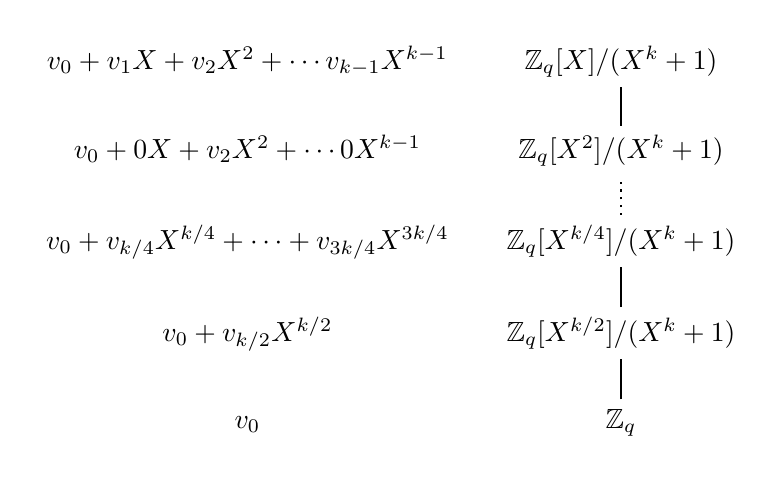
\begin{tikzpicture}[every node/.style={node distance=.7cm}]
        \matrix[matrix of nodes, column sep=0.5cm, row sep=0.5cm]
        {
          $v_0 + v_1 X + v_{2} X^{2} + \cdots v_{k-1} X^{k-1}$ \&
          |(O2k)| $\Z_{q}[X]/(X^{k}+1)$ \\
          % 
          $v_0 + 0 X + v_{2} X^{2} + \cdots 0 X^{k-1}$ \&
          |(Ok)| $\Z_{q}[X^{2}]/(X^{k}+1)$ \\
          %
          $v_{0} + v_{k/4} X^{k/4} + \cdots + v_{3k/4} X^{3k/4}$ \&
          |(O8)| $\Z_{q}[X^{k/4}]/(X^{k}+1)$ \\
          % 
          $v_{0} + v_{k/2} X^{k/2}$ \&
          |(O4)| $\Z_{q}[X^{k/2}]/(X^{k}+1)$ \\
          % 
          $v_{0}$ \&
          |(O2)| $\Z_{q}$ \\ 
        };

        \path
        (Ok) edge[-] (O2k)
        (O8) edge[-,dotted] (Ok)
        (O4) edge[-] (O8)
        (O2) edge[-] (O4)
        ;
      \end{tikzpicture}
    \end{center}

  \item<+-> Homomorphically ``\alert<.>{round}'' $v_{0} \in \Zq$ to
    the message bit $\round{\tfrac{2}{q} \cdot v_{0}} \in \Z_{2}$.

  \end{enumerate}
\end{frame}

\begin{frame}[label=towers]{Algebra: Cyclotomic Towers and Product Bases}
  \begin{itemize}
  \item<+-> Let $\zeta = \zeta_{k}$ have order $k$, a power of 2.  Its
    min.~poly: $\zeta^{k/2}+1=0$.

    \onslide<+-> \medskip So $\O_{k} = \Z[\zeta] \cong
    \Z[X]/(X^{k/2}+1)$ has $\Z$-basis $\set{1,\zeta, \zeta^{2},
      \ldots, \zeta^{k/2-1}}$.

    \bigskip
  \item<+-> \alert<.-.(1)>{Tower} of quadratic extensions
    $\O_{k}/\O_{k/2}/\cdots/\O_{4}/\Z$:
    \onslide<+->
    \begin{center}
      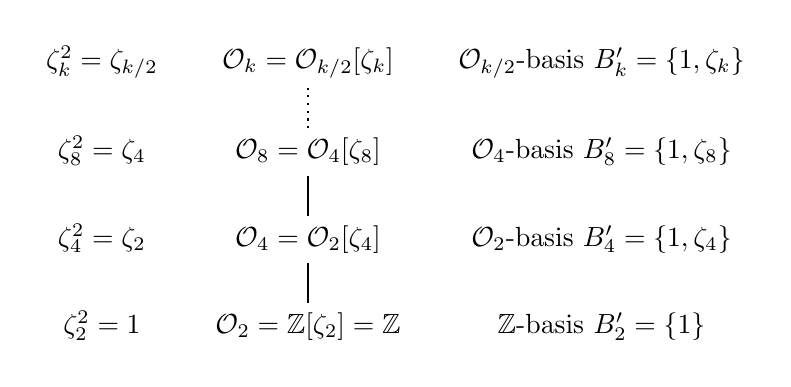
\begin{tikzpicture}[every node/.style={node distance=.7cm}]
        \matrix[matrix of nodes, column sep=0.5cm, row sep=0.5cm]
        {
          $\zeta_{k}^{2} = \zeta_{k/2}$ \&
          |(Ok)| $\O_{k} = \O_{k/2}[\zeta_{k}]$ \&
          $\O_{k/2}$-basis $B'_{k} = \set{1,\zeta_{k}}$ \\
          %
          $\zeta_{8}^{2} = \zeta_{4}$ \&
          |(O8)| $\O_{8} = \O_{4}[\zeta_{8}]$ \&
          $\O_{4}$-basis $B'_{8} = \set{1,\zeta_{8}}$ \\
          %
          $\zeta_{4}^{2} = \zeta_{2}$ \&
          |[] (O4)| $\O_{4} = \O_{2}[\zeta_{4}]$ \&
          $\O_{2}$-basis $B'_{4} = \set{1,\zeta_{4}}$ \\
          %
          $\zeta_{2}^{2} = 1$ \&
          |[] (O2)| $\O_{2} = \Z[\zeta_{2}] = \Z$ \&
          $\Z$-basis $B'_{2} = \set{1}$ \\ 
        };

        \path
        (O8) edge[-,dotted] (Ok)
        (O4) edge[-] (O8)
        (O2) edge[-] (O4)
        ;
      \end{tikzpicture}
    \end{center}

  \item<+-> ``\alert<.>{Product}'' $\Z$-basis of $\O_{k}$:
    \[ B_{k} := B'_{k} \cdot B_{k/2} = B'_{k} \cdot
    B'_{k/2} \cdots B'_{2} = \set{1,\zeta, \zeta^{2}, \ldots,
      \zeta^{k/2-1}}. \]
  \end{itemize}
\end{frame}

\begin{frame}[label=trace]{Algebra: The Trace}
  \begin{itemize}
  \item<+-> Tower of quadratic extensions
    $\O_{k}/\O_{k/2}/\cdots/\O_{4}/\Z$, where $\zeta_{i}^{2} =
    \zeta_{i/2}$.

    \medskip
  \item<+-> $\O_{i}$ has exactly two automorphisms that fix
    $\O_{i/2}$: $\zeta_{i} \mapsto \pm\, \zeta_{i}$.

    \medskip The \alert{trace} function $\trace \colon \O_{i} \to
    \O_{i/2}$ simply sums these automorphisms.

    \medskip

  \item<+-> Let $v = v_{0} \cdot 1 + v_{1} \cdot \zeta_{i} \in \O_{i}$
    for $v_{0}, v_{1} \in \O_{i/2}$.

    \medskip Then $\trace(v) = 2 \cdot v_{0}$.  So $\trace(\O_{i}) = 2
    \cdot \O_{i/2}$.

    \medskip
  \item<+-> More generally, $\trace_{\O_{i}/\O_{i'}}$ sums the
    automorphisms of $\O_{i}$ that fix $\O_{i'}$.

    \smallskip Key facts:

    \medskip
    \begin{itemize}
    \item<+-> $\trace_{\O_{i}/\O_{i''}} = \trace_{\O_{i'}/\O_{i''}}\,
      \circ\, \trace_{\O_{i}/\O_{i'}}$

      \bigskip
    \item<+->[$\Rightarrow$] $\trace_{\O_{i}/\O_{i'}}(\O_{i}) =
      \deg(\O_{i}/\O_{i'}) \cdot \O_{i'}$.

      \bigskip
    \item<+->[$\Rightarrow$] $\trace_{\O_{i}/\Z}(v) = \tfrac{i}{2}
      \cdot v_{0}$, where $v_{0} \in \Z$ is the coeff of
      $\zeta_{i}^{0}=1$.
    \end{itemize}
  \end{itemize}
\end{frame}

\begin{frame}[label=unpacked]{Bootstrapping Unpacked Ciphertexts: Overview}
  \onslide<+-> Recall: $R=\O_{k}$, and $v = c_{0} + c_{1} \cdot s
  \approx \tfrac{q}{2} \mu \in R_{q}$ for message $\mu \in
  \alert<.>{\Z_{2}} \subseteq R_{2}$.

  \smallskip 
  \begin{enumerate}
  \item<+-> \alert<.-.(1)>{Prepare}:
    \begin{itemize}
    \item View $c$ as a ``noiseless'' encryption of plaintext
      \[ \alert<.>{v} = \tfrac{q}{q} \cdot v + 0 = c_{0} + c_{1} \cdot
      s \in \alert<.>{R_{q}}. \]
      Plaintext ring is now $R_{q}$, not $R_{2}$!

      \onslide<+-> \medskip
    \item (Switch to larger ciphertext modulus $Q \gg q$ and ring
      $\tilde{R} \supseteq R$, to support upcoming homomorphic
      operations.)
    \end{itemize}

    \smallskip
  \item<+-> \alert<.>{Extract ``constant term''} $v_{0} \in \Zq$ of
    $v$: homomorphically evaluate
    \[ \frac{\trace_{R/\Z}(v)}{\deg(R/\Z)} = v_{0} \approx
    \tfrac{q}{2} \cdot \mu \in \Zq. \]

    Fast, increases noise rate by only $\approx \sqrt{k}$ factor.

    \medskip
  \item<+-> \alert<.>{Round}: homomorphically evaluate
    $\round{v_{0}} = \mu \in \Z_{2}$.

    \medskip Uses algebraic procedure of depth $\lg(q/2)$ \& size
    $\lg^{2}(q/2)$ {\footnotesize [GHS'12b]}

    \smallskip
  \item<+->[$\star\star$] Now have an encryption of $\round{v_{0}} =
    \mu$. Done!
  \end{enumerate}
\end{frame}

\begin{frame}[label=trace]{Evaluating Trace$_{R/\Z}$ Homomorphically}
  \begin{itemize}
  \item<+->[??] Use ``ring switching'' {\footnotesize [GHPS'12]} ?

    \begin{itemize}
    \item[\GreenCheck] Computes $\trace_{R/R'}$ homomorphically, by
      taking $\trace_{R/R'}$ of ciphertext.

      \smallskip
    \item<+->[\RedCross] Requires hardness of ring-LWE in $R'$ \ldots
      but here $R' = \Z$.
    \end{itemize}

    \medskip
  \item<+->[??] Directly apply all automorphisms $\tau$ of $R/\Z$
    to ciphertext, then sum?
    \begin{itemize}
      \item[] \vspace{-6pt}
        \[ \tau(c_{0}) + \tau(c_{1}) \cdot \tau(s) = \tau(v)
        \quad \stackrel{\text{key-switch}}{\Longrightarrow} \quad
        c'_{0} + c'_{1} \cdot s \approx \tau(v) \]
      \item<+->[\RedCross] $k/2$ automorphisms \& key-switches:
        quadratic work \& space
    \end{itemize}
    
    \medskip
  \item<+->[\GreenCheck] Iteratively ``trace down'' $R=\O_{k} \to
    \O_{k/2} \to \cdots \to \Z$.
    
    \begin{itemize}
    \item<+-> Only need to apply the \alert<.>{two} automorphisms of
      each $\O_{i}/\O_{i/2}$.

    \item<.-> Total $\lg(k)$ automorphisms \& key-switches
      $\Rightarrow \tilde{O}(k)$ work.

      \medskip
    \item<+->[Detail \#1:] ciphertexts are over $\tilde{R} \supseteq
      R$, so use automorphisms of $\tilde{R}$ that coincide with those
      of $\O_{i}/\O_{i/2}$.

      \medskip
    \item<+->[Detail \#2:] each $\trace(\O_{i}) = 2\O_{i/2}$, so lift
      to plaintext modulus $2q$, then halve result.
    \end{itemize}
  \end{itemize}
\end{frame}

% \begin{frame}[label=msb]{Rounding $\Zq$ to $\Z_{2}$, Homomorphically}
%   \begin{algorithmic}[1]
%     \Require Element $x \in \Z_{q}$, where $q=2^{\ell}$
%     \Ensure $\round{x}_{2} \in \Z_2$
%     \State $w_0 \gets x$ \Comment{$w_{0} \in \Zq$}
%     \For{$i \gets 1, \ldots, \ell-1$}
%     \State $y \gets x$ \Comment{$y \in \Zq$, $y = x \pmod*{2^{i+1}}$}
%     \For{$j \gets 0,\ldots, i-1}$
%     \State $w_{j} \gets w_{j}^2$ \label{step:square}
%     \Comment{now $w_{j} = \lsb(\floor{x/2^{j}}) \pmod*{2^{i-j+1}}$}
%     \State $y \gets (y - w_{j})/2 \bmod (q/2^{j+1})$ \label{step:halve}
%     \Comment{now $y \in \Z_{q/2^{j+1}}$,
%       $y = \floor{x/2^{j+1}} \pmod*{2^{i-j}}$}
%     \EndFor
%     \State $w_i \gets y$ \Comment{$w_{i} \in \Z_{q/2^{i}}$,
%       $w_{i} = \floor{x/2^{i}} \pmod{2}$}
%     \EndFor
%     \State \Return $w_{r-1} \in \Z_{2}$
%   \end{algorithmic}

% \end{frame}

\begin{frame}[c,label=main]
  \begin{center}
    {\LARGE \structure{Main Result:\\ \medskip Bootstrapping Packed Ciphertexts}}
  \end{center}
\end{frame}

\begin{frame}[label=packed]{Bootstrapping Packed Ciphertexts: Overview}
  \begin{enumerate}
  \item<+-> \alert<.>{Prepare}: as before, view $c$ as a ``noiseless''
    encryption of plaintext
    \[ v = c_{0} + c_{1} \cdot s = \sum_{j} v_{j} \cdot
    {\color{Blue}b_{j}} \in {\color{Blue}R_{q}}. \] Recall: $\mu =
    \round{v} = \sum_{j} \round{v_{j}} \cdot {\color{Blue}b_{j}} \in
    R_{2}$ (where ${\color{Blue}b_{j}} = \zeta^{j}$).

    \bigskip
  \item<+-> \alert<.>{Homomorphically map} coeffs $v_{j}$ to
    ``$\Zq$-slots'' of certain ring ${\color{Red}S_{q}}$:
    \[ \sum v_{j} \cdot {\color{Blue}b_{j}} \in {\color{Blue}R_{q}}
    \quad \longmapsto \quad \sum v_{j} \cdot {\color{Red}c_{j}} \in
    {\color{Red}S_{q}}. \] {\footnotesize (Change of basis, analogous
      to homomorphic DFT.)}

    \bigskip
  \item<+-> \alert<.>{Batch-round}: homom'ly apply $\round{\cdot}$ on
    all $\Zq$-slots at once {\footnotesize [SV'11]}:
    \[ \sum v_{j} \cdot {\color{Red}c_{j}} \in {\color{Red}S_{q}}\quad
    \longmapsto \quad \sum \round{v_{j}} \cdot {\color{Red}c_{j}} \in
    {\color{Red}S_{2}}. \]

    \medskip
  \item<+-> Homomorphically \alert{reverse-map} $\Z_{2}$-slots back to
    $\color{Blue}B$-coeffs:
    \[ \sum \round{v_{j}} \cdot {\color{Red}c_{j}} \in
    {\color{Red}S_{2}} \quad \longmapsto \quad \sum \round{v_{j}}
    \cdot {\color{Blue}b_{j}} = \mu \in {\color{Blue}R_{2}}. \]
    {\footnotesize (Akin to homomorphic DFT$^{-1}$.)}
  \end{enumerate}
\end{frame}

\begin{frame}[label=slots]{Algebra: Slots and CRT Sets}
  \begin{itemize}
  \item<+-> Let $1=\ell_{0} | \ell_{1} | \ell_{2} | \cdots$ (all odd),
    and $S^{(i)} = \O_{\ell_{i}} = \Z[\zeta_{\ell_{i}}]$. % (degree
                                                      % $\varphi(\ell_{i})$).

    \medskip Identifying $\zeta_{\ell_{i}}^{\ell_{i}/\ell_{i-1}} =
    \zeta_{\ell_{i-1}}$, we get a tower $S^{(i)}/S^{(i-1)}/\cdots/\Z$.

    \medskip 
  \item<+-> In $S=S^{(i)}$, $2$ factors
    into % $\varphi(\ell_{i})/\text{ord}_{\ell_{i}}(2)$
    distinct prime ideals, like so:
    \begin{center}
      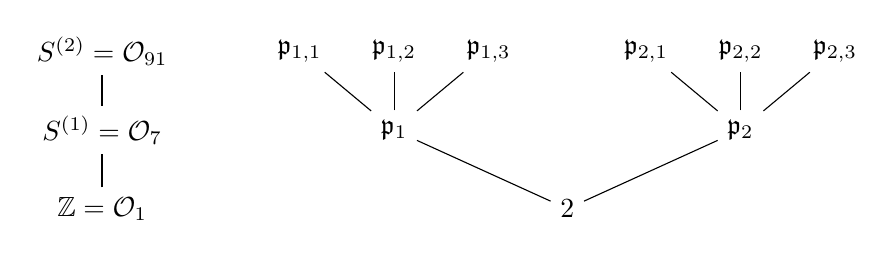
\begin{tikzpicture}[
        level 1/.style={grow via three points={%
            one child at (0,1) and two children at (-2.2,1) and (2.2,1)}},
        level 2/.style={grow via three points={%
            one child at (0,1) and two children at (-.6,1) and (.6,1)}}]
        \node (two) {$2$} [grow'=up]
        child {node (p1) {$\frakp_{1}$}
          child {node (p11) {$\frakp_{1,1}$}}
          child {node {$\frakp_{1,2}$}}
          child {node {$\frakp_{1,3}$}}
        }
        child {node {$\frakp_{2}$}
          child {node {$\frakp_{2,1}$}}
          child {node {$\frakp_{2,2}$}}
          child {node {$\frakp_{2,3}$}}
        }
        ;
        \node[left=5cm of two] (Z) {$\Z = \O_{1}$};
        \node at (p1 -| Z) (S1) {$S^{(1)} = \O_{7}$};
        \node at (p11 -| Z) (S2) {$S^{(2)} = \O_{91}$};
        \path (Z) edge[-] (S1) (S1) edge[-] (S2);
      \end{tikzpicture}
    \end{center}

  \item<+-> By Chinese Rem Thm, $S_{2} \cong \bigoplus_{j}\,
    (S/\frakp_{j})$ via natural homomorphism.

    \onslide<+->
    \medskip ``\alert<.>{CRT set}:'' $C=\set{c_{j}} \subset S$
    s.t.~$c_{j} = 1 \pmod*{\frakp_{j}}$, $= 0 \pmod*{\frakp_{\neq
        j}}$.

    \medskip Mapping $v_{j} \in \Z_{2} \mapsto v_{j} \cdot c_{j} \in
    S_{2}$ embeds $\Z_{2}$ into \alert<.>{$j$th ``slot''} of $S_{2}$.

    \medskip
  \item<+-> Can \alert<.>{factor} $C_{i} = C'_{i} \cdot C_{i-1}$: let
    $c'_{k} = 1 \pmod*{\frakp_{\star,k}}$, $= 0
    \pmod*{\frakp_{\star,\neq k}}$.

    \medskip
  \item<+-> Similarly for $S_{q} \cong \bigoplus_{j}\,
    (S/\frakp_{j}^{\lg q})$.
  \end{itemize}

\end{frame}

\begin{frame}[label=coeffs-slots]{Mapping Coeffs to Slots: Overview}
  \begin{itemize}
  \item<+-> Choose $\color{Red}S$ so that $\color{Red}S_{q}$ has $\geq
    \deg(R/\Z)$ $\Zq$-slots, via: \[ (v_{j}) \in \Zq^{k/2} \;
    \longmapsto\; \sum v_{j} \cdot {\color{Red}c_{j}} \bmod q \] for
    an appropriate CRT set $\color{Red}C = \set{c_{j}} \subset S$ of
    size $k/2$.

    \smallskip
  \item<+-> \alert<.>{Our goal}: homomorphically map $\sum v_{j} \cdot
    {\color{Blue}b_{j}} \in {\color{Blue}R_{q}} \; \longmapsto\; \sum
    v_{j} \cdot {\color{Red}c_{j}} \in {\color{Red}S_{q}}$.

    \onslide<+-> \medskip Equivalently, evaluate the
    \alert<.>{$\Z$-linear$^{*}$ map} $L \colon {\color{Blue}R} \to
    {\color{Red}S}$ defined by \[
    L({\color{Blue}b_{j}})={\color{Red}c_{j}}. \]
    %
    \begin{tikzpicture}[remember picture,overlay]
      \path (current page.south west) node[anchor=south
      west,font=\footnotesize] (Zlinear) {$^{*}\Z$-linear:
        $L(b+b')=L(b)+L(b')$, $L(v \cdot b) = v \cdot L(b)$ for any
        $b,b' \in R, v \in \Z$.};
    \end{tikzpicture}
    %
    \vspace{-20pt}
  \item<+-> \alert<.>{Ring-switching} {\footnotesize [GHPS'12]} lets
    us eval any $R'$-linear map $L \colon {\color{Blue}R} \to R'$

    \onslide<+-> \smallskip \hfill \ldots but only for a
    \alert<.>{subring} $R' \subseteq {\color{Blue}R}$.
  \end{itemize}

  \onslide<+->
  \begin{exampleblock}{Goal for Remainder of Talk}
    \begin{itemize}
    \item Extend ring-switching to (efficiently) handle
      \alert<.>{$\Z$-linear} maps $L \colon {\color{Blue}R} \to
      {\color{Red}S}$.
    \end{itemize}
  \end{exampleblock}
\end{frame}

\begin{frame}[label=solution1]{Algebra: Combining Cyclotomic Rings}
  \begin{itemize}
  \item<+-> Let $\color{Blue}R=\O_{k}$, $\color{Red}S=\O_{\ell}$.  Let
    $d=\gcd(k,\ell)$ and $\color{Purple}m=\lcm(k,\ell)$.

    \onslide<+-> 
    \begin{center}
      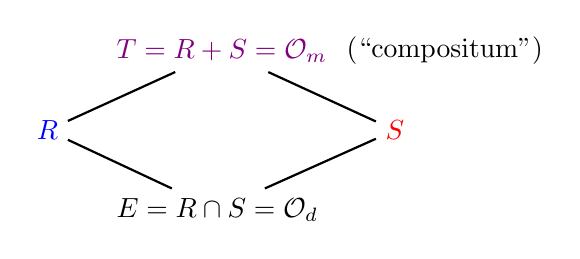
\begin{tikzpicture}[every node/.style={node distance=.7cm}]
        \node (R) {$\color{Blue}R$};
        \node[above right=of R] (T) {$\color{Purple}T = R+S = \O_{m}$};
        \node[below right=of R] (E) {$E = R \cap S = \O_{d}$};
        \node[below right=of T] (S) {$\color{Red}S$};

        \node[anchor=west] at (T.east) {(``compositum'')};
        % \node[anchor=west] at (E.east) {``largest common subring''};

        \path
        (R) edge[-] (E)
        (R) edge[-] (T)
        (E) edge[-] (S)
        (T) edge[-] (S)
        ;
      \end{tikzpicture}
    \end{center}

  \item<+-> Compositum $\color{Purple}T$ as a \alert<.>{tensor
      product} of ${\color{Blue}R},{\color{Red}S}$, where $\otimes$ is
    $E$-bilinear:
  \end{itemize}
  \onslide<.->
  \[ {\color{Purple}T} \cong ({\color{Blue}R}/E) \otimes
  ({\color{Red}S}/E) := \set*{ \sum e_{i,j} ({\color{Blue}r_{i}}
    \otimes {\color{Red}s_{j}}) : e_{i,j} \in E, {\color{Blue}r_{i}
      \in R}, {\color{Red}s_{j} \in S}}. \]

  \onslide<+->
  \begin{block}{Easy Lemma}
    \begin{itemize}
    \item For any $E$-linear $L \colon {\color{Blue}R} \to
      {\color{Red}S}$, there is an $\color{Red}S$-linear $\bar{L}
      \colon {\color{Purple}T} \to {\color{Red}S}$ that agrees with
      $L$ on ${\color{Blue}R}$.

    \item<+-> Proof: define $\bar{L}$ by $\bar{L}({\color{Blue}r}
      \otimes {\color{Red}s}) = L({\color{Blue}r}) \cdot
      {\color{Red}s} \in {\color{Red}S}$.
    \end{itemize}
  \end{block}
\end{frame}

\begin{frame}[label=enhance1]{Enhanced Ring-Switching: First Attempt}
  \begin{itemize}
  \item<+-> Let $\color{Blue}R=\O_{k}$, $\color{Red}S=\O_{\ell}$ be
    s.t.~$\gcd(k,\ell)=1$, $\color{Purple}\lcm(k,\ell)=k\ell$.
    
    \onslide<+->
    \begin{center}
     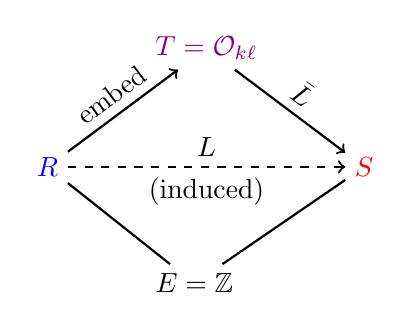
\begin{tikzpicture}[every node/.style={node distance=1.4cm}]
        \node (R) {$\color{Blue}R$};
        \node[above right=of R] (T) {$\color{Purple}T = \O_{k\ell}$};
        \node[below right=of R] (E) {$E = \Z$};
        \node[below right=of T] (S) {$\color{Red}S$};
        
        \path
        (R) edge[-] (E)
        (R) edge[->] node[above,sloped] {embed} (T)
        (E) edge[-] (S)
        (T) edge[->] node[above,sloped] {$\bar{L}$} (S)
        (R) edge[->,dashed] node[above] {$L$} node[below] {(induced)} (S)
        ;
      \end{tikzpicture}
    \end{center}
    
  \item<+-> To homom'ly eval.~$\Z$-linear $L \colon {\color{Blue}R}
    \to {\color{Red}S}$ on an encryption of $v \in R_{q}$,
    
    \onslide<+->
    \begin{enumerate}
    \item Trivially embed ciphertext ${\color{Blue}R} \to
      {\color{Red}T}$ (still encrypts $v$).  \smallskip
    \item Homomorphically apply $\color{Red}S$-linear $\bar{L} \colon
      {\color{Purple}T} \to {\color{Red}S}$ using ring-switching.
      \smallskip
    \item[\GreenCheck] We now have an encryption of $\bar{L}(v) =
      L(v)$ !
    \end{enumerate}

  \item<+->[\RedCross\RedCross] Problem: degree of $\color{Purple}T$
    is \alert<.>{quadratic}, therefore so is runtime \& space.

    \onslide<+->
    This is \alert<.>{inherent} if we treat $L$ as a generic
    $\Z$-linear map!
  \end{itemize}
\end{frame}

\begin{frame}[label=enhance2]{Enhanced Ring-Switching, Efficiently}
  \begin{exampleblock}{Key Ideas}
    \begin{itemize}
    \item<+-> The $\Z$-linear $L \colon {\color{Blue}R} \to
      {\color{Red}S}$ given by $L({\color{Blue}B})={\color{Red}C}$ is
      ``\alert<.>{highly structured},'' because
      ${\color{Blue}B},{\color{Red}C}$ are product sets.
    \item<+-> \alert<.>{Gradually} map $\color{Blue}B$ to
      $\color{Red}C$ through a sequence of ``\alert<.>{hybrid rings}''
      $H^{(i)}$,

      via $E^{(i)}$-linear functions that each send a factor of
      $\color{Blue}B$ to one of $\color{Red}C$.
    \item<+-> Ensure \alert<.>{small compositums}
      $\color{Purple}T^{(i)}=H^{(i-1)} + H^{(i)}$ via \alert{large
        gcd's}: replace prime factors of $\color{Blue}k$ with those of
      $\color{Red}\ell$, one at a time.
    \end{itemize}
  \end{exampleblock}

  \onslide<2->
  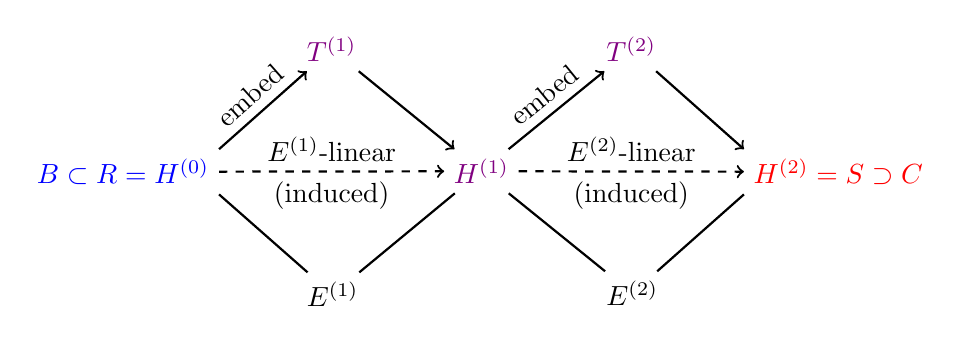
\begin{tikzpicture}[every node/.style={node distance=1.4cm}]
    \node (H0) {$\color{Blue}B \subset R=H^{(0)}$};
    \node[above right=of H0] (T1) {$\color{Purple}T^{(1)}$};
    \node[below right=of H0] (E1) {$E^{(1)}$};
    \node[below right=of T1] (H1) {$\color{Purple}H^{(1)}$};

    \node[above right=of H1] (T2) {$\color{Purple}T^{(2)}$};
    \node[below right=of H1] (E2) {$E^{(2)}$};
    \node[below right=of T2] (H2) {$\color{Red}H^{(2)} = S \supset C$};

    \path
    (H0.south east) edge[-] (E1)
    (H0.north east) edge[->] node[above,sloped] {embed} (T1)
    (E1) edge[-] (H1)
    (T1) edge[->] (H1)
    (H0) edge[->,dashed] node[above] {$E^{(1)}$-linear} node[below]
    {(induced)} (H1)
    % 
    (H1) edge[-] (E2)
    (H1) edge[->] node[above,sloped] {embed} (T2)
    (E2) edge[-] (H2.south west)
    (T2) edge[->] (H2.north west)
    (H1) edge[->,dashed] node[above] {$E^{(2)}$-linear} node[below]
    {(induced)} (H2)
    ;
  \end{tikzpicture}
\end{frame}

\begin{frame}[label=example]{Toy Example}
  \begin{itemize}
  \item<+-> $R={\color{Blue}\O_{8}}$, basis ${\color{Blue} B = B'_{8}
      \cdot B'_{4} = \set{1,\zeta_{8}} \cdot \set{1,\zeta_{4}}}$.

    \medskip
  \item<+-> $S={\color{Red}\O_{7 \cdot 13}}$, CRT set ${\color{Red} C
      = C'_{7} \cdot C'_{91} = \set{c_{1}, c_{2}} \cdot \set{c'_{1},
        c'_{2}, c'_{3}}}$.
  \end{itemize}

  \onslide<+->
  \bigskip
  \begin{center}
    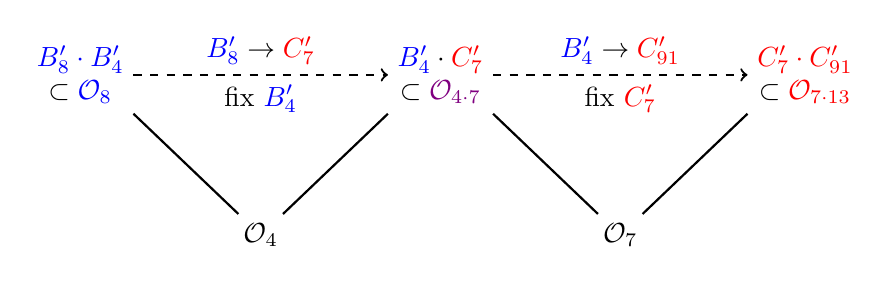
\begin{tikzpicture}[every node/.style={node distance=1.8cm}]
      \node[align=center] (H0)
      {${\color{Blue}B'_{8} \cdot B'_{4}}$\\$\subset {\color{Blue}\O_{8}}$};
      % \node[above right=of H0] (T1) {$\O_{8 \cdot 7}$};
      \node[below right=of H0] (E1) {$\O_{4}$};
      \node[above right=of E1,align=center] (H1)
      {${\color{Blue}B'_{4}} \cdot {\color{Red}C'_{7}}$
        \\$\subset {\color{Purple}\O_{4 \cdot 7}}$};

      % \node[above right=of H1] (T2) {$\O_{4 \cdot 7 \cdot 13}$};
      \node[below right=of H1] (E2) {$\O_{7}$};
      \node[above right=of E2,align=center] (H2) {${\color{Red}C'_{7}
          \cdot C'_{91}}$\\$\subset {\color{Red}\O_{7 \cdot 13}}$};

      \path
      % (H0.north east) edge (T1)
      (H0.south east) edge[-] (E1)
      (E1) edge[-] (H1.south west)
      % (T1) edge[->] (H1.north west)
      (H0) edge[->,dashed] node[below] {fix ${\color{Blue}B'_{4}}$}
      node[above] {${\color{Blue}B'_{8}} \to {\color{Red}C'_{7}}$} (H1)
      % 
      % (H1.north east) edge (T2)
      (H1.south east) edge[-] (E2)
      (E2) edge[-] (H2.south west)
      % (T2) edge[->] (H2.north west)
      (H1) edge[->,dashed] node[below] {fix ${\color{Red}C'_{7}}$}
      node[above] {${\color{Blue}B'_{4}} \to {\color{Red}C'_{91}}$} (H2)
      ;
    \end{tikzpicture}
  \end{center}

  \onslide<+->
  \begin{itemize}
  \item In general, switch through $\leq
    \log(\deg({\color{Blue}R}/\Z)) = \log(\lambda)$ hybrid rings, one
    for each prime factor of $\color{Blue}k$.
  \end{itemize}
\end{frame}

\begin{frame}[label=conclusions]{Final Thoughts}

  \begin{itemize}
  \item<+-> Gradually converting $\color{Blue}B$ to $\color{Red}C$ via
    hybrid rings is roughly analogous to a log-depth FFT butterfly
    network.

    \medskip
  \item<+-> Technique should also be useful for homomorphically
    evaluating other signal-processing transforms having ``sparse
    decompositions.''

    \medskip 
  \item<+-> Practical implementation and evaluation are underway.
  \end{itemize}

  \bigskip
  \onslide<+->
  \begin{center}
    {\Large Thanks!}
  \end{center}
  
\end{frame}

\end{document}

%%% Local Variables: 
%%% mode: latex
%%% TeX-master: t
%%% End: 
